%%%%%%%%%%%%%%%%%%%%%%%%%%%%%%%%%%%%%%%%%%%%%%%%%%%%%%%%%%%%%%%%
%                                                              %
%   USULAN PENELITIAN TESIS (TEMPLATE RESMI KOLOKIUM)          %
%   Magister Ilmu Komputer - Universitas Teknokrat Indonesia   %
%                                                              %
%   Format 1:1 Replikasi Dokumen Word:                         %
%   "Usulan Penelitian Kolokium.docx"                          %
%   - Shading Header Hijau Word (#92D050)                      %
%   - Margin 1 Inci (2.54 cm) Seluruh Sisi                     %
%   - Badan Isi Terbungkus Kotak Berbingkai (Table Grid)       %
%   - Tanpa Mengubah Isi Substantif Dokumen                    %
%                                                              %
%   Peneliti: Amri Reza Wahyudin (NPM: 25321019)               %
%   Pembimbing: Dr. Rohmat Indra Borman, M.Kom.                %
%                                                              %
%%%%%%%%%%%%%%%%%%%%%%%%%%%%%%%%%%%%%%%%%%%%%%%%%%%%%%%%%%%%%%%%

\documentclass[letterpaper,12pt,oneside]{article}

% ---- Packages ----
\usepackage[T1]{fontenc}
\usepackage[utf8]{inputenc}
\usepackage{mathptmx} % Times New Roman
\usepackage[letterpaper,margin=1in]{geometry} % Ukuran Letter & Margin 1 inci persis seperti Word
\usepackage{setspace}
\usepackage{graphicx}
\usepackage{amsmath,amssymb}
\usepackage{booktabs}
\usepackage{array}
\usepackage{tabularx}
\usepackage{ragged2e}
\usepackage[hidelinks]{hyperref}
\usepackage{xurl}
\usepackage[style=ieee,backend=bibtex]{biblatex}
\DeclareLanguageMapping{bahasa}{english}
\addbibresource{refs.bib}
\usepackage[bahasa]{babel}
\usepackage{caption}
\usepackage[most]{tcolorbox}
\usepackage{indentfirst}
% ---- Warna Hijau Resmi Template Word (#92D050) ----
\definecolor{wordgreen}{HTML}{92D050}

% ---- Formatting & Typography ----
\setstretch{1.15} % Kerapatan spasi di dalam kotak tabel Word
\setlength{\parindent}{1.27cm}
\setlength{\parskip}{0pt} % Nol parskip di luar kotak agar antarkotak menempel rapat

% ---- Lingkungan Kotak Bab Word (Breakable tcolorbox) ----
\newtcolorbox{wordsection}[2]{
  breakable,
  enhanced,
  sharp corners,
  colframe=black,
  colback=white,
  colbacktitle=wordgreen,
  coltitle=black,
  boxrule=0.6pt,
  titlerule=0.6pt,
  left=4mm, right=4mm, top=3.5mm, bottom=3.5mm,
  fonttitle=\normalsize,
  title={\textbf{#1}\par\vspace{0.2em}\textit{\small #2}},
  nobeforeafter,
  width=\textwidth,
  before upper={\setlength{\parindent}{1.27cm}\setlength{\parskip}{0.35em}}
}

\newcommand{\subheading}[2]{%
  \par\vspace{0.8em}\noindent
  \textbf{#1. #2}\par\vspace{0.3em}
}

\begin{document}

% ==============================================================
% HALAMAN SAMPUL (COVER) SESUAI TEMPLATE RESMI
% ==============================================================
\begin{titlepage}
  \begin{center}
    \vspace*{0.2cm}

    {\fontsize{14pt}{18pt}\selectfont\bfseries PENGEMBANGAN MODEL ALGORITMA GENETIKA HIBRIDA ADAPTIF DENGAN PENCARIAN LOKAL ELIT UNTUK OPTIMASI PENJADWALAN PERKULIAHAN\par}

    \vspace{0.8cm}

    {\fontsize{14pt}{18pt}\selectfont\bfseries USULAN PENELITIAN TESIS\par}

    \vspace{0.8cm}

    
\includegraphics[width=3.6cm]{figures/logo_ut.png}

    \vspace{0.8cm}

    {\fontsize{12pt}{16pt}\selectfont Diajukan sebagai salah satu syarat untuk Kolokium\\[0.2em]
    Program Studi Magister Ilmu Komputer\par}

    \vspace{0.9cm}

    {\fontsize{14pt}{18pt}\selectfont\bfseries Amri Reza Wahyudin}\\[0.2em]
    {\fontsize{14pt}{18pt}\selectfont\bfseries 25321019}

    \vspace{0.8cm}

    {\fontsize{12pt}{16pt}\selectfont\bfseries Pembimbing: Dr. Rohmat Indra Borman, M.Kom.\par}

    \vfill

    {\fontsize{14pt}{18pt}\selectfont\bfseries PROGRAM STUDI MAGISTER ILMU KOMPUTER\\[0.2em]
    FAKULTAS TEKNIK DAN ILMU KOMPUTER\\[0.2em]
    UNIVERSITAS TEKNOKRAT INDONESIA\\[0.2em]
    BANDAR LAMPUNG\\[0.2em]
    2026\par}

  \end{center}
\end{titlepage}

\pagenumbering{arabic}
\setcounter{page}{1}

% ==============================================================
% 1. JUDUL
\noindent\begin{wordsection}{A. JUDUL}{Tuliskan judul usulan penelitian maksimal 20 kata}
\textbf{Pengembangan Model Algoritma Genetika Hibrida Adaptif dengan Pencarian Lokal Elit untuk Optimasi Penjadwalan Perkuliahan}

\vspace{0.3em}
\noindent\textit{Judul Bahasa Inggris: Development of a Hybrid Adaptive Genetic Algorithm Model with Elite Local Search for University Course Timetabling Optimization (14 kata)}
\end{wordsection}%
\vspace{-1.2pt}%
\noindent\begin{wordsection}{B. RINGKASAN}{Isian ringkasan penelitian tidak lebih dari 300 kata yang berisi urgensi, tujuan, metode, dan hasil yang diharapkan}
Penjadwalan perkuliahan (\textit{University Course Timetabling Problem} / UCTP) merupakan persoalan optimasi kombinatorial berstatus \textit{NP-hard} dengan kompleksitas ruang pencarian faktorial $\mathcal{O}(n!)$. Di Program Studi Ilmu Komputer Universitas Muhammadiyah Metro, penyusunan jadwal masih dilakukan secara manual menggunakan lembar kerja berulang yang memakan waktu 2--3 hari kerja serta rawan memicu bentrokan ruangan dan dosen. Algoritma Genetika (GA) konvensional dengan parameter statis rentan mengalami konvergensi prematur dan terjebak pada optimum lokal. Penelitian terdahulu oleh Pamungkas dan Neta~\cite{pamungkas2025saga} mengusulkan \textit{Self-Adaptive Genetic Algorithm} (SAGA) berbasis \textit{fuzzy logic} dan \textit{cooperative coevolution}; namun mekanisme tersebut memunculkan trade-off kompleksitas inferensi tinggi dan osilasi parameter di generasi lanjut. Penelitian ini bertujuan merancang dan memvalidasi model \textit{Hybrid Adaptive Genetic Algorithm} (HAGA) untuk UCTP. HAGA mengintegrasikan dua mekanisme saling melengkapi: (1) kontrol parameter adaptif deterministik (\textit{Adaptive Parameter Control} / APC) berbasis metrik keragaman genotipik \textit{normalized pairwise Hamming distance} ($H_{\text{norm}}$) dengan pembatasan jepit eksplisit (\textit{clamping}), dan (2) \textit{Elite Local Search} (ELS) berbasis \textit{stochastic first-improvement hill climbing} yang menargetkan kuliah berkonflik pada 10\% individu terbaik di bawah paritas anggaran evaluasi global ($B_{\max}$). Metode penelitian eksperimental menguji HAGA terhadap tiga algoritma pembanding berlingkungan setara (Canonical GA, PSO, dan SA) melintasi 21 instance tolok ukur internasional ITC 2007 CB-CTT, data riil UM Metro, dan dataset sintetis. Pengujian pra-penelitian awal pada instance ITC 2007 \texttt{comp01} mengonfirmasi kelayakan komputasi model, di mana HAGA mencapai tingkat kelayakan solusi 100\% ($HCV=0$) berbanding 0\% pada GA kanonikal, serta menghasilkan perbaikan penalti kendala lunak yang signifikan secara statistik ($p = 0{,}00195$ pada uji Wilcoxon). Kontribusi penelitian ini mencakup formulasi integrasi kontrol parameter keragaman linier dan pencarian lokal elit yang transparan, isolasi kontribusi komponen melalui studi ablasi empat tahap, serta protokol evaluasi komputasi berparitas adil.
\end{wordsection}%
\vspace{-1.2pt}%
\noindent\begin{wordsection}{C. PENDAHULUAN}{Pendahuluan penelitian terdiri dari latar belakang, rumusan permasalahan yang akan diteliti, pertanyaan penelitian, tujuan, manfaat penelitian dan kerangka teoritis (state of the art) tidak lebih dari 1500 kata. Sitasi disusun dan ditulis berdasarkan sistem IEEE.}

\subheading{1}{Latar Belakang}

Penjadwalan perkuliahan di perguruan tinggi merupakan salah satu persoalan manajemen operasional paling krusial sekaligus menantang. Setiap semester, pengelola akademik diwajibkan mengalokasikan ratusan kegiatan perkuliahan ke dalam kombinasi ruang kuliah dan slot waktu yang terbatas dengan mematuhi batasan fisik serta preferensi institusional. Dalam literatur sains komputasi, permasalahan ini diformulasikan sebagai \textit{University Course Timetabling Problem} (UCTP) yang terbukti bersifat \textit{NP-hard}~\cite{qu2009survey,mccollum2009setting}. Kompleksitas ruang kombinatorial tumbuh secara eksponensial seiring bertambahnya jumlah kelas, ruangan, dan preferensi dosen.

Kondisi operasional pada Program Studi Ilmu Komputer Universitas Muhammadiyah Metro menunjukkan bahwa proses penyusunan jadwal masih bertumpu pada metode manual berbasis Microsoft Excel~\cite{mustika2025penerapan}. Pendekatan ini menuntut waktu kerja 2 hingga 3 hari kerja penuh dan sangat rentan terhadap kelalaian manusia (\textit{human error}), seperti tabrakan jadwal mengajar dosen atau pemesanan ganda (\textit{double-booking}) ruang kuliah. Kendala dalam UCTP terbagi menjadi dua kategori fundamental:
\begin{enumerate}
    \item \textbf{Kendala Kaku (\textit{Hard Constraints}):} Batasan fisik mutlak yang wajib dipenuhi tanpa toleransi, seperti ketiadaan jadwal bentrok untuk dosen, ruangan, maupun kurikulum mahasiswa pada jam yang sama. Pelanggaran kendala kaku (\textit{Hard Constraint Violation} / HCV) menyebabkan jadwal tidak layak (\textit{infeasible}) digunakan.
    \item \textbf{Kendala Lunak (\textit{Soft Constraints}):} Preferensi mutu pedagogis dan kenyamanan operasional, seperti kesesuaian kapasitas ruang kuliah, minimalisasi sebaran jam kosong mahasiswa, serta pemenuhan preferensi hari mengajar dosen. Pelanggaran kendala lunak (\textit{Soft Constraint Violation} / SCV) mengukur tingkat inefisiensi kualitas jadwal.
\end{enumerate}

Algoritma Genetika (GA) telah lama dieksplorasi sebagai metaheuristik utama untuk menyelesaikan UCTP di Indonesia~\cite{sari2019optimasi,kristiadi2019genetic,fachrie2021paralelisasi}. Namun, GA konvensional memiliki kelemahan mendasar: probabilitas persilangan (\textit{crossover rate}, $P_c$) dan probabilitas mutasi (\textit{mutation rate}, $P_m$) bersifat statis sepanjang generasi evolusi~\cite{eiben1999parameter,karafotias2015parameter}. Parameter statis memicu dilema eksplorasi-eksploitasi: nilai mutasi yang konstan rendah menyebabkan hilangnya keragaman alel secara cepat menuju konvergensi prematur pada optimum lokal yang belum bebas bentrok, sedangkan nilai mutasi tinggi yang konstan merusak struktur kromosom unggul yang telah terbentuk.

Untuk mengatasi kelemahan tersebut, Pamungkas dan Neta~\cite{pamungkas2025saga} mengajukan \textit{Self-Adaptive Genetic Algorithm} (SAGA) dengan memadukan \textit{fuzzy logic} dan \textit{cooperative coevolution}. SAGA melaporkan kepuasan kendala 98,9\% pada studi kasus institusionalnya. Namun, desain arsitektur SAGA memunculkan trade-off komputasi yang berat: waktu komputasi rata-rata mencapai 31 menit, variabilitas antareksekusi tinggi (koefisien variasi 8,59\%), serta timbulnya osilasi nilai parameter di generasi tinggi yang justru memperburuk fenomena stagnasi lokal~\cite{pamungkas2025saga}. Kondisi ini menegaskan perlunya alternatif kontrol adaptif yang beroperasi secara lebih langsung, deterministik, dan efisien tanpa kompleksitas aturan kabur (\textit{fuzzy rule base}). Analisis kesenjangan antara harapan teoritis, realita operasional, dan dampak disajikan pada Tabel~\ref{tab:harapan_realita}.

\begin{center}
\captionof{table}{Analisis Harapan terhadap Realita, Problem, dan Dampak}
\label{tab:harapan_realita}
\small
\begin{tabularx}{\linewidth}{>{\RaggedRight\arraybackslash}p{3.5cm} >{\RaggedRight\arraybackslash}X >{\RaggedRight\arraybackslash}X >{\RaggedRight\arraybackslash}X}
\toprule
\textbf{Ekspektasi} & \textbf{Realita} & \textbf{Problem} & \textbf{Dampak} \\
\midrule
Jadwal kuliah tersusun otomatis, cepat, dan bebas konflik. & Penyusunan jadwal di UM Metro masih manual berbasis Excel. & Belum ada sistem optimasi komputasi cerdas yang diterapkan. & Butuh 2--3 hari kerja, boros tenaga staf, dan rawan jadwal bentrok. \\[0.4em]
GA menghasilkan solusi optimal global secara konsisten. & GA konvensional memakai parameter statis ($P_c, P_m$). & Parameter statis memicu konvergensi dini dan stagnasi lokal. & Terjebak pada jadwal yang masih melanggar kendala kaku ($HCV > 0$). \\[0.4em]
GA adaptif mampu menyesuaikan dinamika evolusi secara lincah. & Metode adaptif SAGA memakai sistem inferensi fuzzy multi-input. & Kompleksitas fuzzy memicu overhead inferensi dan osilasi parameter. & Eksekusi lambat (rata-rata 31 menit) dan variabilitas solusi tinggi. \\[0.4em]
Model optimasi tervalidasi secara objektif dan terstandarisasi. & Mayoritas riset UCTP domestik hanya diuji pada satu data lokal. & Ketiadaan evaluasi pada benchmark internasional standar. & Tingkat keandalan dan generalisasi algoritma tidak dapat diukur. \\
\bottomrule
\end{tabularx}
\end{center}

\subheading{2}{State of the Art}

Kajian literatur komputasi evolusioner telah membuktikan bahwa efektivitas metaheuristik bergantung pada pengelolaan parameter~\cite{eiben1999parameter,karafotias2015parameter,lacerda2021systematic}. Eiben dkk.~\cite{eiben1999parameter} membagi kontrol parameter ke dalam tiga ranah: deterministik, adaptif (berbasis umpan balik populasi), dan \textit{self-adaptive} (parameter dikodekan ke dalam gen). Cicirello~\cite{cicirello2016genetic} menunjukkan bahwa kontrol adaptif mengungguli parameter tetap pada persoalan penjadwalan industri.

Dalam domain penjadwalan akademik, berbagai hibridisasi telah dirancang untuk memperkuat kemampuan eksploitasi GA. Amrulloh dan Sela~\cite{amrulloh2021optimasi} mengombinasikan GA dengan \textit{Tabu Search} untuk pembagian ruangan perkuliahan. Badoni dkk.~\cite{badoni2023exploration} menerapkan hibrida GA dan \textit{Iterated Local Search} (ILS) pada persoalan UCTP kurikulum. Song dkk.~\cite{song2021competition} mengusulkan \textit{competition-guided multi-neighborhood local search} yang mencapai performa sangat kompetitif pada 15 dari 21 instance tolok ukur kompetisi internasional ITC 2007. Di ranah multi-objektif, Ghaffar dkk.~\cite{ghaffar2021multi} mengembangkan \textit{Multi-Objective Fuzzy Adaptive Memetic Algorithm} (MO-FAMA) yang menggabungkan kontrol fuzzy dengan \textit{hill climbing} dan \textit{tabu search}. Han dan Wang~\cite{han2025gradual} membuktikan keunggulan hibridisasi GA dengan pemrograman dinamis untuk alokasi ruang.

Terkait pencarian lokal pada individu elit, Kurniawan dkk.~\cite{kurniawan2025elite} mendemonstrasikan bahwa penerapan \textit{hill climbing} secara selektif pada kromosom peringkat teratas (\textit{elite individuals}) dengan skema pembelajaran Lamarckian secara signifikan mampu mereduksi penalti jadwal kuliah di institusi Indonesia. Sementara itu, Sakal, Fieldsend, dan Keedwell~\cite{sakal2023genotype} mengevaluasi metrik keragaman genotipik berbasis jarak Hamming pada instance kompetisi ITC 2007 Track 3 dan menemukan bahwa jarak Hamming antar kromosom merupakan indikator paling efektif untuk mendeteksi wilayah plateau dalam ruang pencarian UCTP. Pemetaan komparatif posisi HAGA terhadap metode-metode tersebut dirangkum dalam Matriks Diferensiasi pada Tabel~\ref{tab:matriks_diferensiasi}.

\begin{center}
\captionof{table}{Matriks Diferensiasi Arsitektur HAGA terhadap Pendekatan Literatur}
\label{tab:matriks_diferensiasi}
\footnotesize
\begin{tabularx}{\linewidth}{>{\RaggedRight\arraybackslash}X *{5}{>{\centering\arraybackslash}p{1.9cm}}}
\toprule
\textbf{Dimensi Perancangan} & \textbf{HAGA} & \textbf{SAGA~\cite{pamungkas2025saga}} & \textbf{Kurniawan~\cite{kurniawan2025elite}} & \textbf{Ghaffar~\cite{ghaffar2021multi}} & \textbf{Canonical GA} \\
\midrule
Kontrol Parameter Adaptif Linier ($H_{\text{norm}}$) & \checkmark & --- & --- & --- & --- \\
Sistem Inferensi Fuzzy Dinamis & --- & \checkmark & --- & \checkmark & --- \\
Pencarian Lokal Elit Generasional (ELS) & \checkmark & \checkmark & \checkmark & \checkmark & --- \\
Penargetan Konflik Terarah (\textit{Conflict-Directed}) & \checkmark & --- & --- & --- & --- \\
Evaluasi Benchmark Internasional (ITC 2007) & \checkmark & --- & --- & --- & --- \\
Protokol Paritas Anggaran Evaluasi ($B_{\max}$) & \checkmark & --- & --- & --- & --- \\
Isolasi Komponen via Studi Ablasi 4-Tahap & \checkmark & --- & --- & --- & --- \\
Validasi Statistik Inferensial (30 Run) & \checkmark & \checkmark & --- & --- & --- \\
\bottomrule
\end{tabularx}
\end{center}

\subheading{3}{Research Gap}

Berdasarkan telaah mendalam terhadap literatur mutakhir, teridentifikasi empat celah penelitian (\textit{research gap}) yang menjadi landasan usulan penelitian ini:
\begin{enumerate}
    \item \textbf{Gap 1 -- Ketiadaan Aturan Kontrol Parameter Linier Berbasis Keragaman Pasangan untuk UCTP:} Sebagian besar pendekatan adaptif pada UCTP mengandalkan sistem inferensi fuzzy yang membutuhkan penyusunan basis aturan subjektif dan komputasi inferensi berlapis di setiap generasi. Belum ada penelitian yang menerapkan aturan transfer linier deterministik langsung tertutup (\textit{closed-form formula}) berbasis jarak Hamming ternormalisasi berpasangan ($H_{\text{norm}}$) yang dilengkapi pembatasan rentang aman (\textit{clamping bounds}) untuk mengendalikan probabilitas $P_c$ dan $P_m$ secara simultan.
    \item \textbf{Gap 2 -- Kelemahan Pengendalian Paritas Anggaran Komputasi pada Hibridisasi Metaheuristik:} Studi terdahulu yang menggabungkan GA dengan pencarian lokal (seperti Kurniawan dkk.~\cite{kurniawan2025elite}) tidak menerapkan akuntansi evaluasi objektif bersama. Hal ini memunculkan kerancuan apakah keunggulan solusi yang diperoleh murni berasal dari sinergi algoritma atau sekadar dampak dari pemberian jatah evaluasi komputasi ekstra pada tahapan pencarian lokal.
    \item \textbf{Gap 3 -- Ketiadaan Evaluasi Multi-Korpus Terstandarisasi pada Studi UCTP Domestik:} Riset UCTP di Indonesia mayoritas diuji terbatas pada satu dataset lokal institusi masing-masing tanpa mengikutsertakan instance tolok ukur internasional yang diakui komunitas ilmiah (seperti ITC 2007 CB-CTT~\cite{mccollum2009setting}), sehingga tingkat generalisasi algoritma tidak dapat diukur secara objektif.
    \item \textbf{Gap 4 -- Ketiadaan Analisis Ablasi Komponen Secara Terisolasi:} Penelitian hibridisasi terdahulu mengimplementasikan seluruh komponen modifikasi secara bersamaan tanpa menguji secara empiris kontribusi kausal masing-masing komponen pembangun (kontribusi modul adaptif versus kontribusi pencarian lokal elit) melalui rancangan pengujian berparitas ketat.
\end{enumerate}

\subheading{4}{Rumusan Masalah}

Berdasarkan latar belakang dan celah penelitian yang telah diidentifikasi, pertanyaan penelitian (\textit{Research Questions}) yang diajukan adalah:
\begin{enumerate}
    \item \textbf{RQ1:} Apakah HAGA menghasilkan tingkat kelayakan jadwal ($HCV = 0$) dan nilai penalti kendala lunak ($SCV$) yang secara signifikan lebih unggul dibandingkan Canonical GA, PSO, dan SA di bawah paritas anggaran evaluasi ($B_{\max}$) yang setara?
    \item \textbf{RQ2:} Sejauh mana kontribusi empiris masing-masing komponen pembangun HAGA (modul kontrol parameter adaptif APC dan modul pencarian lokal elit ELS) yang diukur melalui studi ablasi empat tahap?
    \item \textbf{RQ3:} Seberapa sensitif kinerja konvergensi dan kualitas solusi HAGA terhadap variasi parameter sensitivitas kemiringan ($\alpha$ dan $\beta$) serta ukuran populasi?
    \item \textbf{RQ4:} Apakah integrasi mekanisme APC dan ELS pada HAGA menghasilkan laju penuntasan kendala kaku yang lebih cepat (generasi konvergensi lebih rendah) dibandingkan metaheuristik baseline?
\end{enumerate}

\subheading{5}{Tujuan Penelitian}

Tujuan yang hendak dicapai melalui penelitian ini meliputi:
\begin{enumerate}
    \item Merancang dan mengimplementasikan arsitektur HAGA dengan mengintegrasikan kontrol parameter adaptif linier berbasis \textit{normalized pairwise Hamming distance} dan \textit{conflict-directed elite local search}.
    \item Mengevaluasi kinerja HAGA terhadap tiga algoritma pembanding (Canonical GA, PSO, SA) menggunakan protokol 30 run independen pada 21 instance benchmark ITC 2007 CB-CTT, data riil UM Metro, dan korpus sintetis.
    \item Mengisolasi dan mengukur kontribusi kausal komponen APC dan ELS melalui studi ablasi empat tahap ($\text{Canonical GA} \to \text{GA+APC} \to \text{GA+ELS} \to \text{HAGA}$).
    \item Melakukan analisis sensitivitas parameter dan dinamika kurva keragaman genotipik untuk membuktikan stabilitas model dalam mencegah konvergensi prematur.
\end{enumerate}

\subheading{6}{Manfaat Penelitian}

\noindent\textbf{Manfaat Teoritis:}
Penelitian ini memberikan kontribusi ilmiah berupa perumusan model kontrol parameter deterministik berbasis keragaman genotipik yang ringan komputasi untuk optimasi kombinatorial berkonstrain ketat. Desain studi ablasi berparitas anggaran menegakkan metodologi eksperimen yang transparan untuk membuktikan efektivitas komponen metaheuristik secara terisolasi.

\noindent\textbf{Manfaat Praktis:}
Bagi Program Studi Ilmu Komputer Universitas Muhammadiyah Metro dan institusi pendidikan tinggi secara umum, algoritma ini menyediakan solusi otomatisasi penyusunan jadwal kuliah yang terbebas dari jadwal bentrok ($HCV = 0$) dalam waktu eksekusi yang efisien dan stabil, menghilangkan beban penyusunan manual tahunan.
\end{wordsection}%
\vspace{-1.2pt}%
\noindent\begin{wordsection}{D. METODOLOGI}{Isian metodologi atau cara untuk mencapai tujuan yang telah ditetapkan tidak lebih dari 1500 kata. Pada bagian metodologi wajib dilengkapi dengan diagram alir penelitian yang menggambarkan alur, metode, dan pendekatan yang digunakan (input -- proses -- output). Format diagram alir dapat berupa file JPG/PNG. Metode penelitian harus memuat sekurang-kurangnya prosedur penelitian, data yang digunakan, metode pengolahan data dan metode analisis.}

\subheading{1}{Prosedur Penelitian}

Penelitian ini dilaksanakan melalui enam tahapan sistematis terstruktur yang membentuk kerangka kerja eksperimental komparatif:
\begin{enumerate}
    \item \textbf{Fase 1 -- Studi Literatur dan Formalisasi Masalah:} Telaah literatur kontrol parameter metaheuristik, perumusan formulasi matematis kendala UCTP, dan penyiapan instance tolok ukur ITC 2007.
    \item \textbf{Fase 2 -- Perancangan dan Implementasi HAGA:} Pengembangan perangkat lunak dalam bahasa Python (NumPy dan SciPy) yang menegakkan kontrak metode: encoding kromosom 1D berindeks event, kalkulasi jarak Hamming ternormalisasi secara berkala, penyesuaian parameter linier terikat, pencarian lokal terarah bentrok pada 10\% individu elit, dan akuntansi pemotongan anggaran evaluasi global.
    \item \textbf{Fase 3 -- Implementasi Algoritma Pembanding Baseline:} Membangun modul pembanding independen dengan representasi, penilai fungsi objektif, dan batas kuota komputasi yang setara: Canonical GA (statis), PSO diskret, dan Simulated Annealing (SA).
    \item \textbf{Fase 4 -- Pelaksanaan Eksperimen Multi-Korpus:} Eksekusi komputasi menggunakan 30 \textit{random seeds} independen melintasi tiga korpus data di bawah invarian paritas anggaran evaluasi fungsi objektif global $B_{\max} = 50.000$ evaluasi per run.
    \item \textbf{Fase 5 -- Studi Ablasi dan Uji Statistik Inferensial:} Mengisolasi kontribusi modul melalui skema empat tahap ($\text{GA} \to \text{GA+APC} \to \text{GA+ELS} \to \text{HAGA}$), dilanjutkan uji signifikansi Wilcoxon signed-rank ($\alpha=0{,}05$), uji peringkat omnibus Friedman, dan analisis post-hoc Nemenyi.
    \item \textbf{Fase 6 -- Dokumentasi dan Diseminasi Ilmiah:} Penyusunan naskah tesis lengkap, persiapan artikel ilmiah untuk jurnal terakreditasi nasional (target SINTA 2), serta publikasi artefak eksperimen terbuka (*open science*) di GitHub.
\end{enumerate}

\subheading{2}{Algoritma HAGA: Kontrak Metode dan Formulasi Matematis}

Algoritma HAGA yang diusulkan bekerja berdasarkan lima kontrak arsitektural yang terdefinisi secara presisi:

\noindent\textbf{1. Representasi Kromosom 1D Berindeks Event:}
Kromosom direpresentasikan sebagai larik satu dimensi berindeks kegiatan kuliah $\mathbf{c} \in \mathbb{N}^E$, dengan panjang gen tepat sama dengan total sesi kuliah $E$. Setiap gen $c_k = (r_k, t_k)$ menyimpan alokasi ruang kuliah $r_k \in \mathcal{R}$ dan slot waktu $t_k \in \mathcal{T}$. Dosen pengampu dan kurikulum melekat tetap pada indeks kegiatan $k$, sehingga pelanggaran relasi dosen dan kurikulum diukur melalui penalti $HCV$ secara transparan.

\noindent\textbf{2. Pengukuran Keragaman Genotipik Populasi ($H_{\text{norm}}$):}
Keragaman genotipik populasi diukur pada setiap awal generasi menggunakan jarak Hamming ternormalisasi berpasangan di seluruh $\frac{N(N-1)}{2}$ kombinasi pasangan individu:
\begin{equation}
    H_{\text{norm}}(t) = \frac{2}{N(N-1)} \sum_{i=1}^{N-1} \sum_{j=i+1}^{N} \left[ \frac{1}{E} \sum_{k=1}^{E} \mathbb{I}(c_{i,k} \neq c_{j,k}) \right]
\end{equation}
di mana $\mathbb{I}(\cdot)$ bernilai $1$ jika penugasan ruang atau waktu berbeda, dan $0$ jika identik. Nilai $H_{\text{norm}}(t) \in [0, 1]$ merefleksikan tingkat dispersi alel dalam populasi.

\noindent\textbf{3. Aturan Kontrol Parameter Adaptif Linier (APC):}
Nilai keragaman $H_{\text{norm}}(t)$ dipetakan secara deterministik untuk memperbarui probabilitas persilangan $P_c(t)$ dan mutasi $P_m(t)$ dengan pembatasan jepit eksplisit (\textit{clamping bounds}):
\begin{align}
    P_c(t) &= \operatorname{clamp}\left( P_{c,\min} + (P_{c,\max} - P_{c,\min}) \cdot H_{\text{norm}}(t), \; [0{,}40, 0{,}95] \right) \\
    P_m(t) &= \operatorname{clamp}\left( P_{m,\max} - (P_{m,\max} - P_{m,\min}) \cdot H_{\text{norm}}(t), \; [0{,}01, 0{,}30] \right)
\end{align}
Saat keragaman menyusut ($H_{\text{norm}} \to 0$), $P_m(t)$ terangkat hingga batas atas $0{,}30$ untuk menginjeksi diversifikasi baru, sementara $P_c(t)$ diredam ke $0{,}40$. Sebaliknya, saat keragaman melimpah ($H_{\text{norm}} \to 1$), $P_c(t)$ ditingkatkan hingga $0{,}95$ untuk memacu eksploitasi blok bangunan unggul.

\noindent\textbf{4. Elite Local Search (ELS) Terarah Konflik:}
Pada setiap generasi, 10\% individu terbaik ($K = 0{,}10 \times N$) menjalani perbaikan lokal berbasis \textit{stochastic first-improvement hill climbing} dengan batas maksimal 50 langkah per individu. ELS mendeteksi perkuliahan yang terlibat bentrokan dan mencoba merelokasikannya ke slot waktu acak. Perubahan langsung diterima seketika apabila fitness membaik (\textit{first-improvement}), dan kromosom yang telah diperbaiki langsung menggantikan individu induk di populasi (\textit{Lamarckian replacement}).

\noindent\textbf{5. Paritas Anggaran Evaluasi Bersama ($B_{\max}$):}
Setiap pemanggilan fungsi evaluasi (baik saat evaluasi populasi offspring maupun dalam langkah pencarian ELS) mencatat dan memotong jatah kuota evaluasi objektif global $B_{\max} = 50.000$. Seluruh algoritma berhenti seketika saat kuota evaluasi terpenuhi.

Alur kerja operasional Algoritma HAGA beserta tahapan intervensi adaptifnya disajikan secara sistematis pada Gambar~\ref{fig:haga_flowchart}.
\begin{center}
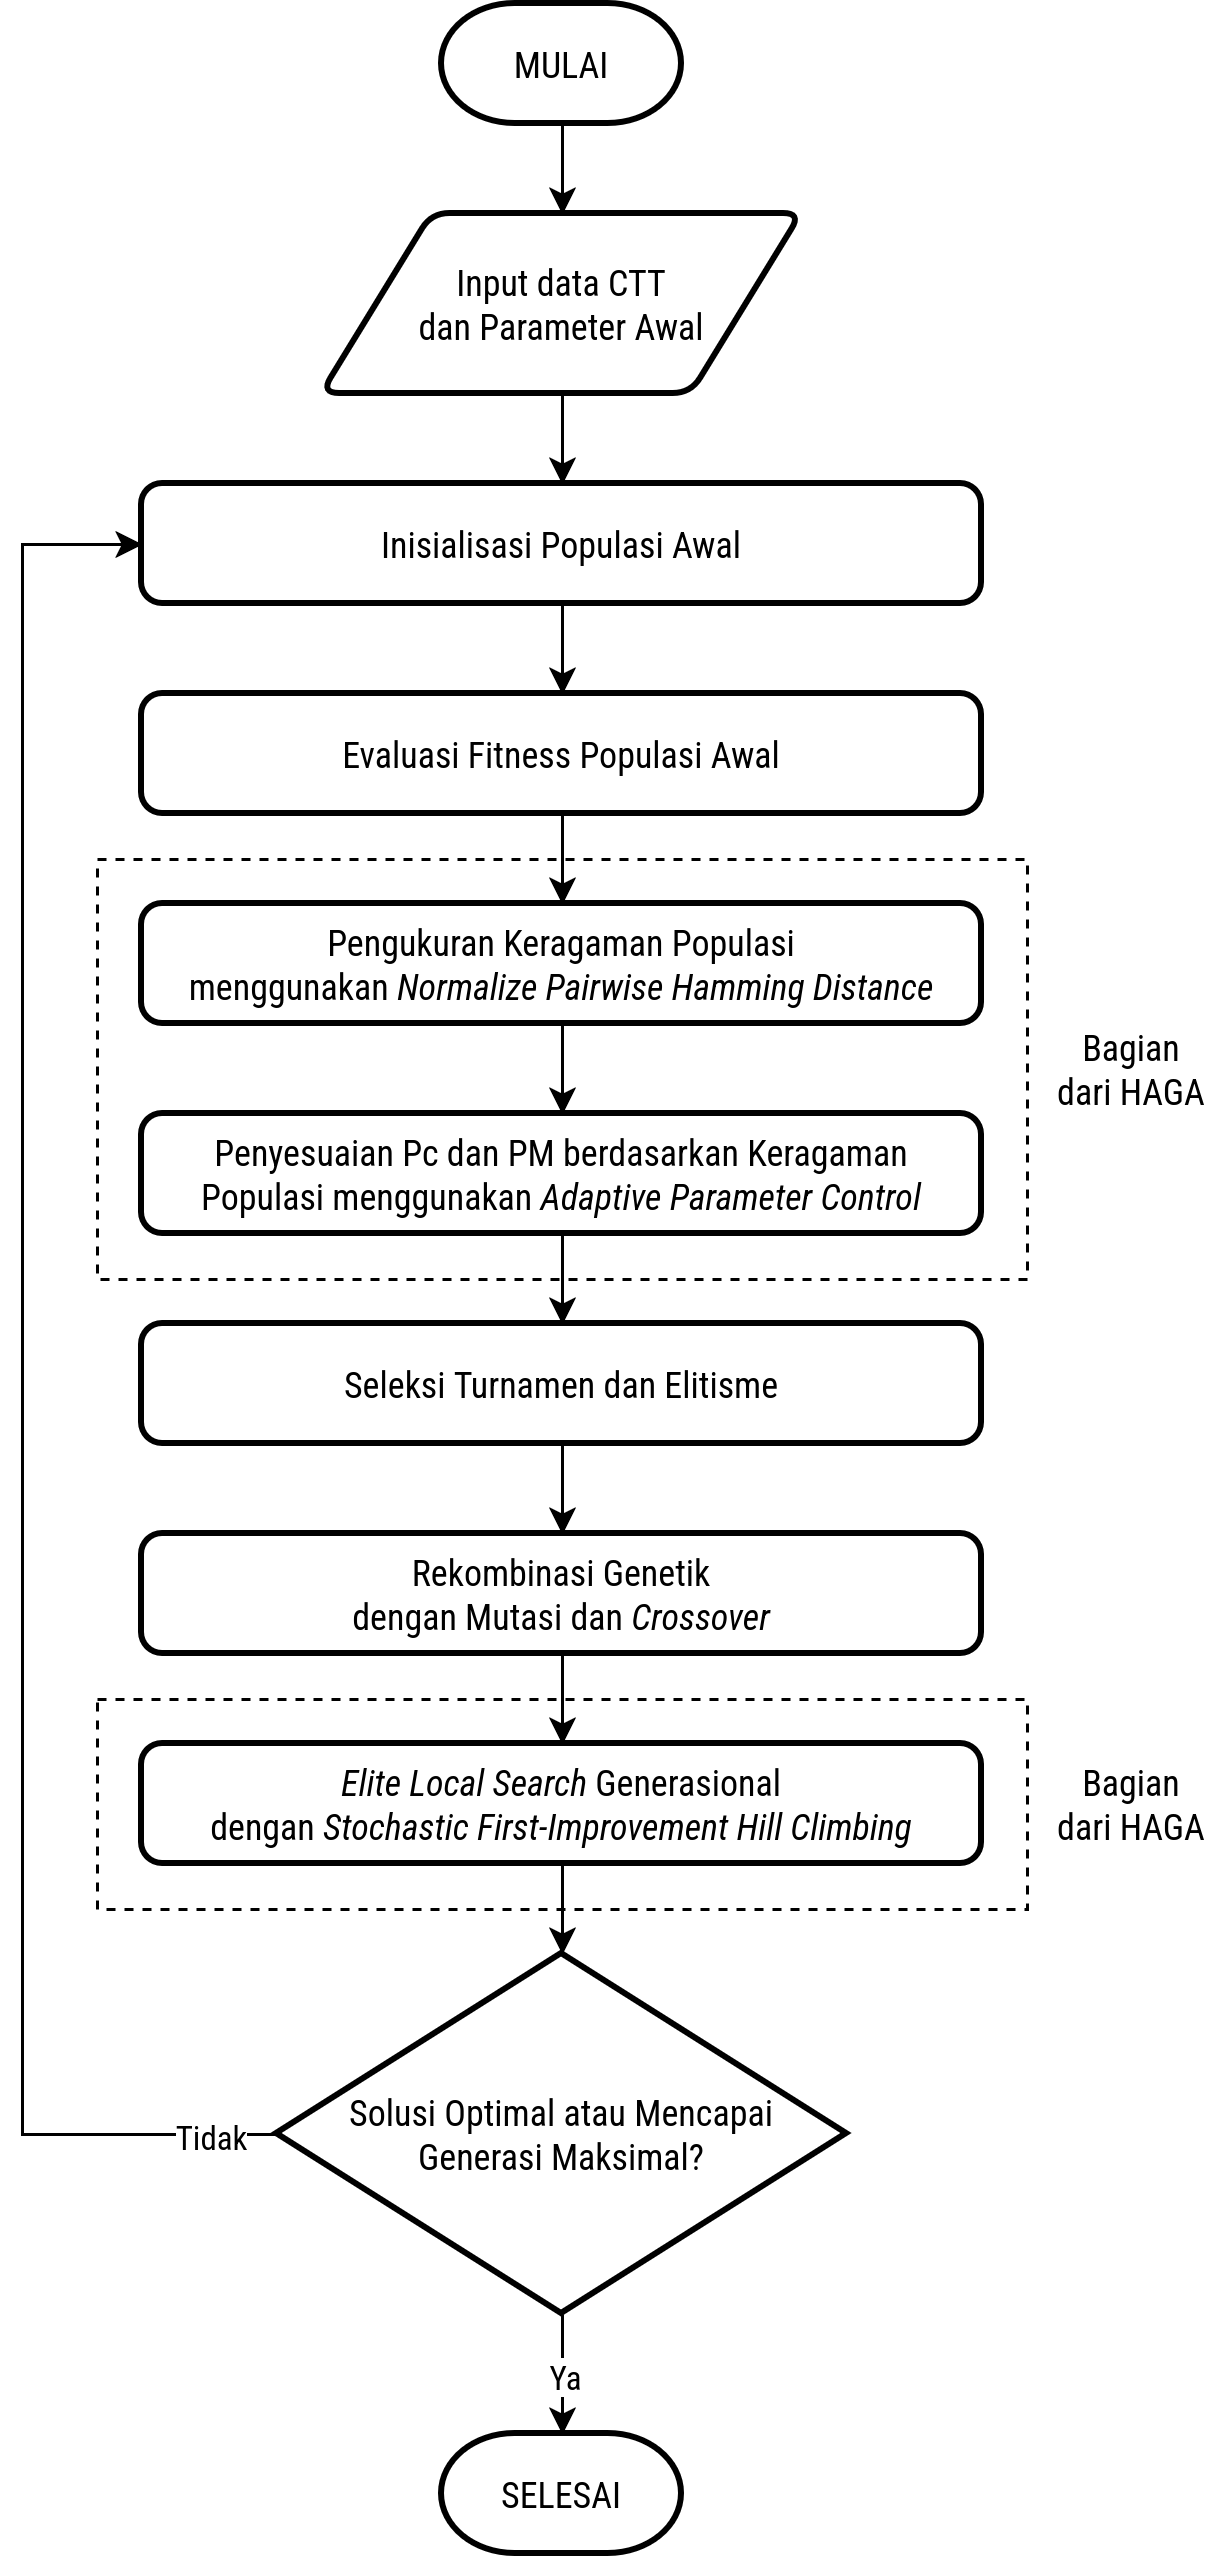
\includegraphics[width=0.68\linewidth,height=9.2cm,keepaspectratio]{figures/haga_algorithm_flowchart.png}
\captionof{figure}{Diagram Alur Algoritma HAGA: Menampilkan Tahapan Inisialisasi, Pengukuran Keragaman, Kontrol Parameter Adaptif, dan Pencarian Lokal Elit}
\label{fig:haga_flowchart}
\end{center}

\subheading{3}{Partisi Korpus Dataset}

Pengujian performa algoritma dilakukan melintasi tiga korpus data yang dievaluasi secara terpisah:
\begin{enumerate}\setlength{\itemsep}{0pt}\setlength{\parsep}{0pt}\setlength{\parskip}{0pt}
    \item \textbf{Korpus Konfirmatori Utama (ITC 2007 CB-CTT):} Sebanyak 21 instance resmi kompetisi internasional (\texttt{comp01}--\texttt{comp21}) yang mencakup variasi 50 hingga 434 kegiatan kuliah, 5 hingga 20 ruang kuliah, dan konstrain kurikulum otentik~\cite{mccollum2009setting}.
    \item \textbf{Studi Kasus Riil (UM Metro):} Data riil operasional Program Studi Ilmu Komputer UM Metro yang mencakup 42 mata kuliah, 19 dosen, 10 ruangan, dan 40 slot waktu mingguan untuk menguji aplikabilitas praktis.
    \item \textbf{Korpus Sintetis (Uji Stres dan Skalabilitas):} Dataset buatan terkontrol yang memvariasikan jumlah mata kuliah ($E \in \{50, 100, 200\}$) dengan utilisasi ruang 70\% guna menguji batas beban komputasi model.
\end{enumerate}

\subheading{4}{Algoritma Pembanding dan Parameter Eksperimen}

HAGA diperbandingkan secara adil terhadap tiga algoritma baseline:
\begin{itemize}\setlength{\itemsep}{0pt}\setlength{\parsep}{0pt}\setlength{\parskip}{0pt}
    \item \textbf{Canonical GA:} Parameter statis ($P_c = 0{,}85, P_m = 0{,}05$), seleksi turnamen ($k=3$), dan \textit{two-point crossover}.
    \item \textbf{Particle Swarm Optimization (PSO):} Bobot inersia $w=0{,}7$, konstanta akselerasi $c_1=c_2=1{,}5$, dengan pemetaan posisi kontinu ke diskret.
    \item \textbf{Simulated Annealing (SA):} Suhu awal $T_0=100$, pendinginan geometrik $\lambda=0{,}95$, dan operator perpindahan acak 1-event.
\end{itemize}

Rangkuman parameter pengujian disajikan pada Tabel~\ref{tab:param_eksperimen}.

\begin{center}
\captionof{table}{Parameter Konfigurasi Pengujian Algoritma}
\label{tab:param_eksperimen}
\small
\begin{tabularx}{\linewidth}{l l >{\RaggedRight\arraybackslash}X}
\toprule
\textbf{Parameter} & \textbf{Nilai Konfigurasi} & \textbf{Keterangan Operasional} \\
\midrule
Ukuran Populasi ($N$) & $50, 100, 200$ & Pengujian analisis sensitivitas \\
Maksimum Evaluasi ($B_{\max}$) & $50.000$ evaluasi & Anggaran bersama mutlak per run \\
Replikasi Independen & 30 run per instance & Pengendalian \textit{random seed} terisolasi \\
Rentang Probabilitas $P_c$ & $[0{,}40, 0{,}95]$ & Batas jepit kontrol adaptif \\
Rentang Probabilitas $P_m$ & $[0{,}01, 0{,}30]$ & Batas jepit kontrol adaptif \\
Ukuran Turnamen & 3 individu & Tekanan seleksi induk \\
Kuota Individu ELS & 10\% individu terbaik & Intensitas eksploitasi lokal \\
Maksimal Langkah ELS & 50 langkah per individu & Pengendalian beban eksploitasi \\
Tingkat Signifikansi ($\alpha$) & $0{,}05$ & Ambang uji hipotesis non-parametrik \\
\bottomrule
\end{tabularx}
\end{center}

\subheading{5}{Metode Pengolahan Data dan Analisis Statistik}

Pengolahan data eksperimen dicatat secara otomatis ke dalam berkas CSV yang merekam: tingkat kelayakan ($HCV=0$), nilai pelanggaran kendala kaku ($HCV$), nilai penalti kendala lunak ($SCV$), nilai fitness skalar gabungan, profil keragaman genotipik $H_{\text{norm}}(t)$, jejak fluktuasi parameter $P_c(t)$ dan $P_m(t)$, serta waktu eksekusi komputasi.

Analisis statistik dilaksanakan melalui:
\begin{enumerate}
    \item \textbf{Uji Komparasi Berpasangan (Wilcoxon Signed-Rank Test):} Membandingkan performa HAGA secara langsung terhadap masing-masing baseline pada tingkat signifikansi $\alpha = 0{,}05$ dengan koreksi \textit{Holm-Bonferroni} untuk mengendalikan tingkat kesalahan tipe I pada hipotesis jamak.
    \item \textbf{Uji Peringkat Multi-Algoritma (Friedman Test \& Nemenyi Post-Hoc):} Menguji signifikansi peringkat global seluruh algoritma melintasi 21 instance tolok ukur ITC 2007, dilengkapi pembuatan diagram \textit{Critical Difference} (CD).
    \item \textbf{Studi Ablasi Empat Tahap:} Mengukur selisih delta performa antar-tahap ($\text{GA} \to \text{GA+APC} \to \text{GA+ELS} \to \text{HAGA}$) untuk membuktikan kontribusi kausal masing-masing komponen pembangun.
\end{enumerate}

\subheading{6}{Hasil Validasi Kelayakan Awal (Hasil Pra-Penelitian)}

Sebagai bukti empiris kesiapan metode, eksperimen pra-penelitian pendahuluan (\textit{preliminary feasibility study}) telah diselesaikan pada instance tolok ukur resmi ITC 2007 \texttt{comp01.ctt} (30 mata kuliah, 6 ruang kelas, 53 konstrain) menggunakan 10 \textit{random seeds} independen di bawah anggaran evaluasi bersama $B_{\max} = 25.000$ evaluasi. Seluruh kode sumber, dataset, dan data mentah pra-penelitian telah dipublikasikan secara terbuka pada repositori: \url{https://github.com/AmZaDin14/haga-uctp}. Rangkuman hasil perbandingan kuantitatif disajikan pada Tabel~\ref{tab:hasil_prapenelitian}.

\begin{center}
\captionof{table}{Hasil Uji Pra-Penelitian: Canonical GA vs HAGA pada ITC 2007 \texttt{comp01}}
\label{tab:hasil_prapenelitian}
\footnotesize
\begin{tabularx}{\linewidth}{>{\RaggedRight\arraybackslash}p{5.4cm} >{\centering\arraybackslash}p{2.6cm} >{\centering\arraybackslash}p{2.6cm} >{\RaggedRight\arraybackslash}X}
\toprule
\textbf{Metrik Evaluasi} & \textbf{Canonical GA} & \textbf{HAGA (Diusulkan)} & \textbf{Selisih ($\Delta$) \& Keterangan} \\
\midrule
Tingkat Kelayakan Solusi ($HCV=0$) & 0\% (0/10) & \textbf{100\% (10/10)} & +100\% (Mutlak Layak) \\[0.3em]
Pelanggaran Kendala Kaku Min ($HCV_{\min}$) & 40 & \textbf{0} & -40 (Bebas Bentrok) \\[0.3em]
Pelanggaran Kendala Kaku Rerata ($HCV_{\text{mean}}$) & $48{,}0 \pm 4{,}6$ & \textbf{0,0} & -48,0 (Jadwal Bebas Bentrok) \\[0.3em]
Kendala Lunak Terbaik ($SCV_{\min}$) & 1.769 & \textbf{1.300} & -469 ($-26{,}5\%$) \\[0.3em]
Kendala Lunak Rerata ($SCV_{\text{mean}}$) & $2.221{,}0 \pm 174{,}8$ & \textbf{1.748{,}0} & -473,0 ($-21{,}3\%$) \\[0.3em]
Waktu Komputasi Rerata & 107,4 detik & \textbf{87,4 detik} & -20,0 detik ($-18{,}6\%$) \\
\midrule
\multicolumn{4}{>{\RaggedRight\arraybackslash}p{\dimexpr\linewidth-2\tabcolsep\relax}}{%
\textbf{Uji Signifikansi Non-Parametrik Wilcoxon Signed-Rank ($N=10$ run independen):}\par
$\bullet$ Penalti Kendala Lunak ($SCV$): $W = 55{,}0, \; p = 0{,}001953 \; (p < 0{,}01)$ $\to$ \textbf{Signifikan secara Statistik}\par
$\bullet$ Fitness Skalar Gabungan ($F(S)$): $W = 55{,}0, \; p = 0{,}000977 \; (p < 0{,}001)$ $\to$ \textbf{Signifikan secara Statistik}} \\
\bottomrule
\end{tabularx}
\end{center}


\subheading{7}{Diagram Alir Penelitian Tahapan (Input -- Proses -- Output)}

Gambar~\ref{fig:tahapan_penelitian} menyajikan diagram alir tahapan pelaksanaan penelitian yang memetakan masukan (\textit{input}), proses riset eksperimental komparatif, dan keluaran (\textit{output}) untuk setiap tahap kegiatan.

\begin{center}
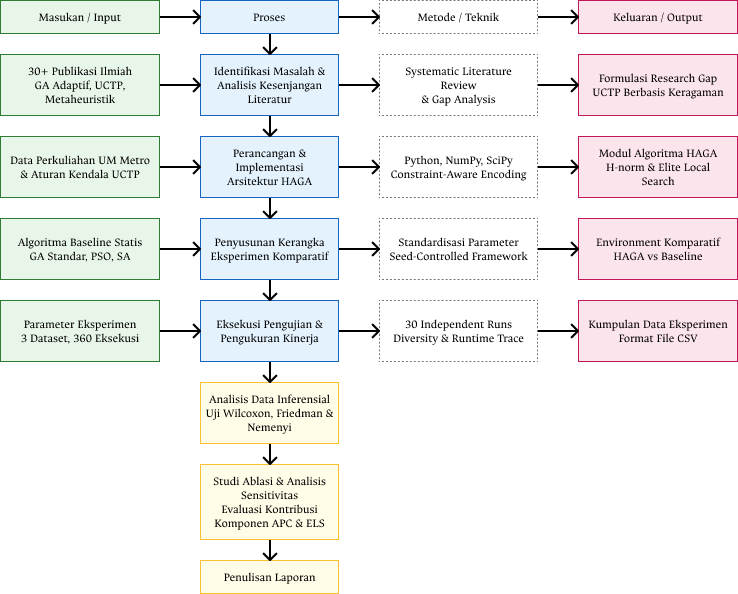
\includegraphics[width=0.82\linewidth]{figures/flowchart.png}
\captionof{figure}{Diagram Alir Tahapan Penelitian Komparatif HAGA (Input -- Proses -- Output)}
\label{fig:tahapan_penelitian}
\end{center}
\end{wordsection}%
\vspace{-1.2pt}%
\noindent\begin{wordsection}{E. HASIL YANG DIHARAPKAN}{Jelaskan hasil yang diharapkan dari penelitian. (Kontribusi Teoritis dan Praktis)}
\noindent\textbf{Kontribusi Teoritis:}
\begin{enumerate}
    \item Formulasi model kontrol parameter deterministik berbasis keragaman genotipik pasangan ternormalisasi ($H_{\text{norm}}$) yang terbukti secara matematis mampu mencegah konvergensi prematur pada optimasi kombinatorial UCTP.
    \item Penegakan protokol pengujian metaheuristik berbasis paritas anggaran evaluasi global bersama ($B_{\max}$) yang mengeliminasi bias keunggulan komputasi tersembunyi pada algoritma hibrida.
    \item Bukti empiris mengenai kontribusi individual komponen adaptif dan pencarian lokal melalui metodologi studi ablasi terisolasi melintasi 21 instance tolok ukur standar internasional.
\end{enumerate}

\noindent\textbf{Kontribusi Praktis:}
\begin{enumerate}
    \item Sistem otomatisasi penjadwalan perkuliahan yang stabil dan terbebas dari jadwal bentrok ($HCV = 0$) untuk diterapkan pada Program Studi Ilmu Komputer Universitas Muhammadiyah Metro.
    \item Repositori kode sumber terbuka (\textit{open science}) berbasis Python yang terdokumentasi lengkap di GitHub (\url{https://github.com/AmZaDin14/haga-uctp}) beserta berkas tolok ukur untuk mendukung keterbukaan dan reproduksibilitas penelitian komputasi.
    \item Artikel ilmiah hasil penelitian yang siap dipublikasikan pada jurnal nasional terakreditasi SINTA 2 atau seminar internasional bereputasi.
\end{enumerate}
\end{wordsection}%
\vspace{-1.2pt}%
\noindent\begin{wordsection}{F. JADWAL PENELITIAN}{Jadwal penelitian disusun berdasarkan pelaksanaan penelitian dan disesuaikan berdasarkan lama bulan pelaksanaan penelitian (minimal 4 bulan)}
Penelitian ini direncanakan berlangsung selama 5 (lima) bulan dengan alokasi kegiatan kerja terstruktur sebagaimana disajikan pada Tabel~\ref{tab:jadwal_penelitian}.

\begin{center}
\captionof{table}{Matriks Jadwal Pelaksanaan Penelitian Tesis (5 Bulan)}
\label{tab:jadwal_penelitian}
\small
\begin{tabularx}{\linewidth}{c >{\RaggedRight\arraybackslash}X *{5}{c}}
\toprule
\textbf{No.} & \textbf{Tahapan Kegiatan Penelitian} & \textbf{Bulan 1} & \textbf{Bulan 2} & \textbf{Bulan 3} & \textbf{Bulan 4} & \textbf{Bulan 5} \\
\midrule
1 & Studi Literatur dan Kajian SLR Sistematis & \checkmark & \checkmark & & & \\
2 & Perancangan dan Implementasi Kode HAGA & & \checkmark & \checkmark & & \\
3 & Implementasi Baseline (GA, PSO, SA) & & & \checkmark & & \\
4 & Pelaksanaan Eksperimen Multi-Korpus (360 Run) & & & \checkmark & \checkmark & \\
5 & Analisis Data, Statistik, dan Studi Ablasi & & & & \checkmark & \checkmark \\
6 & Penulisan Naskah Tesis Lengkap dan Publikasi & & & & \checkmark & \checkmark \\
\bottomrule
\end{tabularx}
\end{center}
\end{wordsection}%
\vspace{-1.2pt}%
\noindent\begin{wordsection}{G. DAFTAR PUSTAKA}{Daftar Pustaka dengan format IEEE}
\printbibliography[heading=none]
\end{wordsection}

\end{document}
